
\documentclass{article}

\usepackage{graphviz}
\usepackage{url}
\usepackage{hyperref}
\usepackage{fullpage}
\usepackage{parskip}
\usepackage{fancyvrb}
\usepackage{amsmath}
\usepackage{framed}

\usepackage{listings}
\lstset{numbers=left,
		basicstyle=\footnotesize,
		captionpos=b,
		xleftmargin=0.3in}

\providecommand{\e}[1]{\ensuremath{\times 10^{#1}}}

\VerbatimFootnotes

\raggedright

% Change enumerate section numbering
\renewcommand*{\theenumii}{\theenumi.\arabic{enumii}}
\renewcommand*{\labelenumii}{\theenumi.\arabic{enumii}}

\begin{document}

% {{{ title page
\vspace*{1.0in}

\centerline{\LARGE \textbf{SprinklerPI}}
%\centerline{(Product Test Plan)}
\vspace{0.3in}
\centerline{\LARGE Product Test Plan}

\vfill

\begin{center}
\begin{tabular}{c}
Jeremiah Mahler \\
EECE 490B, CSU Chico \\
\today
\end{tabular}
\end{center}

\vspace{1in}

\thispagestyle{empty}

%\vfill

\pagebreak
% }}}

\thispagestyle{empty}
\tableofcontents
\clearpage

% {{{ Information Required for Execution
\section{Information Required for Execution}

\subsection{Purpose}

The purpose of this test protocol is to verify the full and complete
operation of the SprinklerPI system.

\subsection{Scope}

This test protocol should be executed to verify that each principal feature
and function performs within specification called out by the engineering
requirements document. In addition, other necessary specifications shall
be tested such as specific and necessary user, installation and power
requirements. The testing called out in this protocol is subject exclusively
to those selected specifications provided for the SprinklerPI.

\subsection{Responsibilities}

It is the responsibility of the assigned test engineer to execute all tests
included herein to the best of their ability. If necessary, seek additional
assistance to execute tasks.

\subsection{References}

Not applicable at this time.

%\subsection{Definitions}

\subsection{Equipment/Supplies}

\begin{itemize}
\item 110 volts AC power supply.
\item Digital volt meter.
\item One Sprinkler valve, residential 270 mA.
\end{itemize}

\subsection{Precautions \& Warnings}

This test plan contains certain warnings, cautions and important
notes that the test engineer must be aware of while performing these tests.
The following illustrates each of these messages and how to recognize them.

\fbox{
\textbf{WARNING: \textless message\textgreater}
}

The ``WARNING: Message'' alerts the user about safety issues that are of
the highest importance, such as possible injury to the operator.

\fbox{
\textbf{CAUTION: \textless message\textgreater}
}

The ``CAUTION: Message'' alerts the user to issues concerning possible
damage to the equipment or that can lead to erroneous test results.

\fbox{
\textbf{IMPORTANT: \textless message\textgreater}
}

The ``IMPORTANT: Message'' alerts the user to important design changes.

% }}}

\section{Testing Features and Functions}

This system has a modular design with a power supply module and from
one to three control/driver modules.
The following test procedure tests each module individually.
After an individual module has been tested and shown to be in working
order it can be used to construct a full system.

% {{{ Power Supply Module
\subsection{Power Supply Module}

\begin{framed}
\textbf{IMPORTANT}: The DC voltage has been changed
from 5V to 3.3V.
The label on version 20140304 of the power supply PCB still
refers to 5V despite this change.
\end{framed}

\begin{figure}[hbp!]
\begin{center}
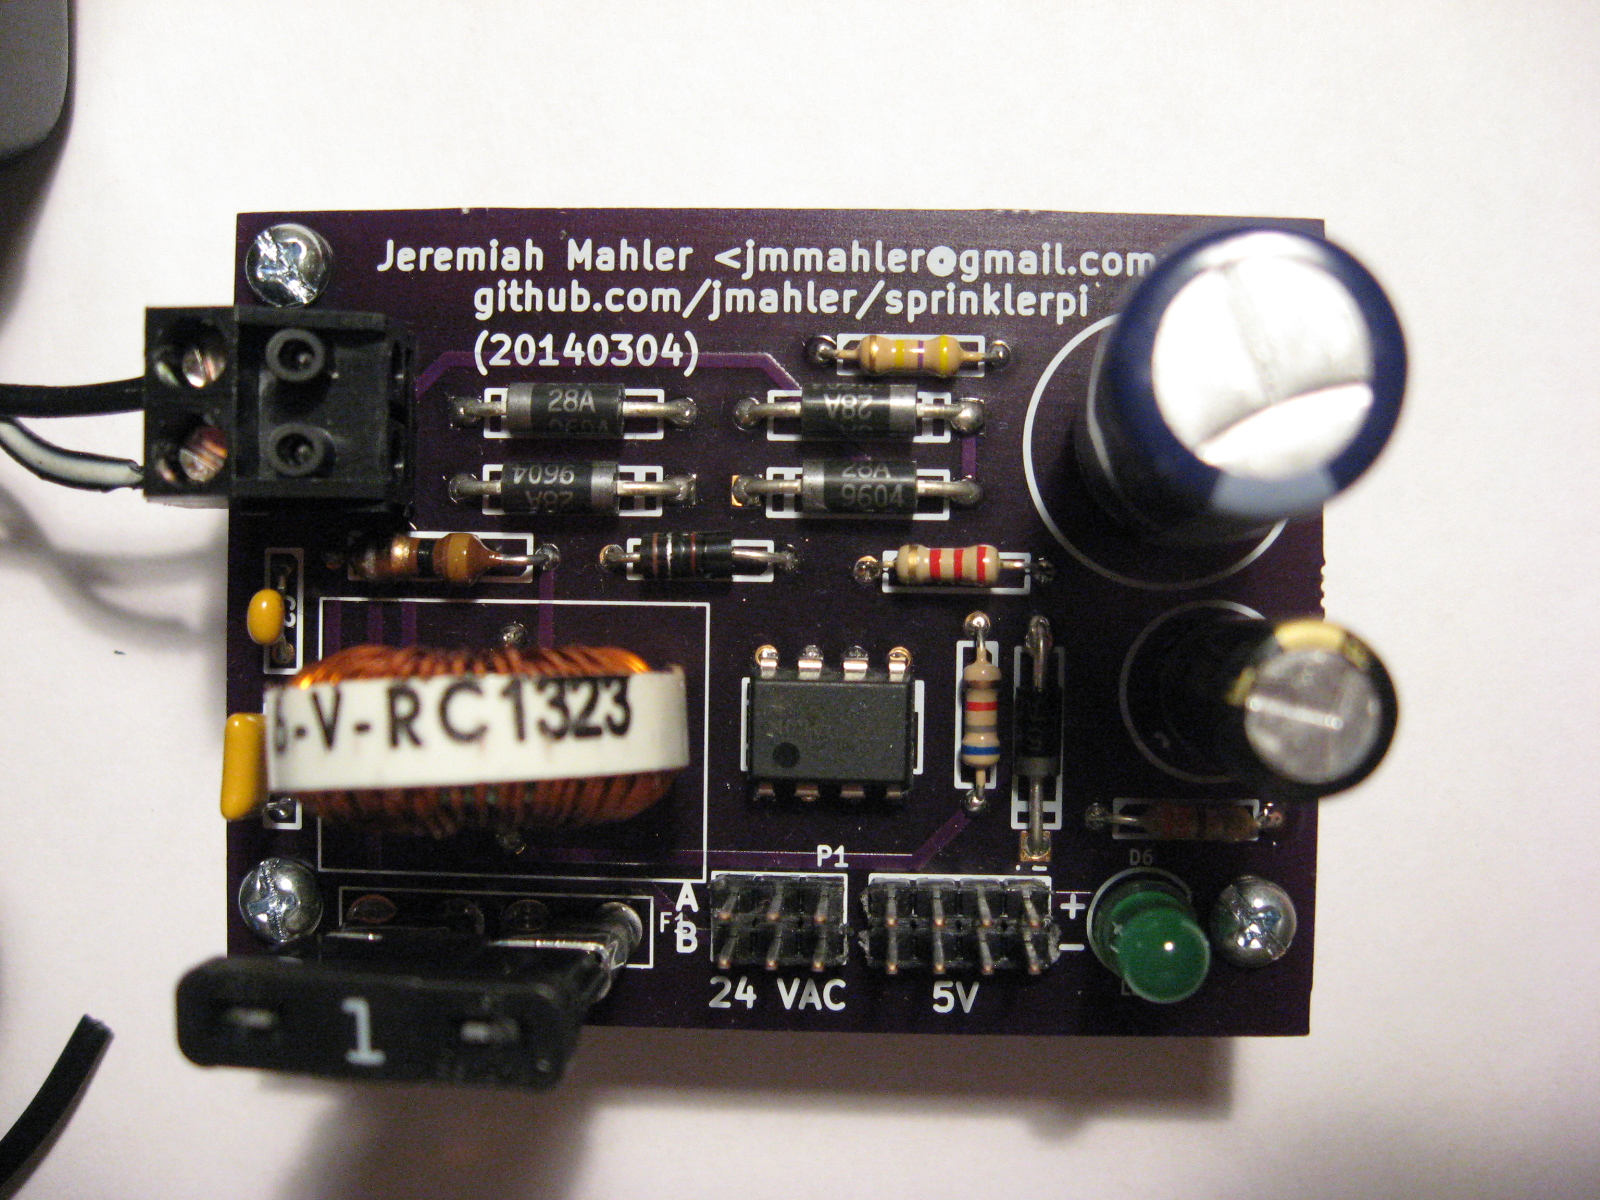
\includegraphics[scale=0.15,angle=0]{img/power_pcb-assembled-02.jpg}
\end{center}
\caption{Assembled power supply module PCB.
The 24 volts AC input is in the top left.
The green power LED is on the bottom right.
The headers for 24 volts AC output and 3.3 volts DC
output are on the bottom.
}\label{fig:psm2}
\end{figure}

\begin{enumerate}
\item Equipment Required
	\begin{itemize}
	\item SprinklerPI power supply module (revision 20140304).
	\item 110 volts AC power supply (standard U.S.).
	\item 110 volts AC to 24 volts AC power adapter.
	\item Digital multi meter.
	\end{itemize}
\item Input
	\begin{itemize}
	\item 24 volts AC from 110 to 24 volts AC adapter.
	\end{itemize}
\item Output
	\begin{itemize}
	\item Green power LED on.
	\item 24$\pm4.8$ (20\%) volts AC output.
	\item 3.3$\pm0.3$ (10\%) volts DC output.
	\end{itemize}
\pagebreak
\item Test Description \\

The 110 volt to 24 volt AC power adapter should be connected to the
two pin input header (Figure \ref{fig:psm2}, top left) and screwed down.
With the power adapter plugged in to a 110 volts AC power supply the
green power LED should come on.
Using a DMM to measure voltage, there should be 3.3 volts DC output on
the ``5V'' header pins and 24 volts AC output on the ``24 VAC'' header pins.
Be sure to switch from AC to DC modes on the DMM as necessary.
The polarity of DC voltages are denoted on the PCB (Figure \ref{fig:psm2}).

\item Test Results \\
	\vspace{0.2in}
	\begin{tabular}{|l|l|l|l|}
		\hline
		& Value & Pass/Fail & Results/Data\hspace{2in} \\
		\hline
		Power LED on? &&& \\
		\hline
		$24\pm4.8$ volts AC &&& \\
		\hline
		$3.3\pm0.3$ volts DC &&& \\
		\hline
	\end{tabular}
\end{enumerate}
% }}}

% {{{ Control/Driver
\clearpage
\subsection{Control/Driver}

\begin{figure}[htbp!]
\begin{center}
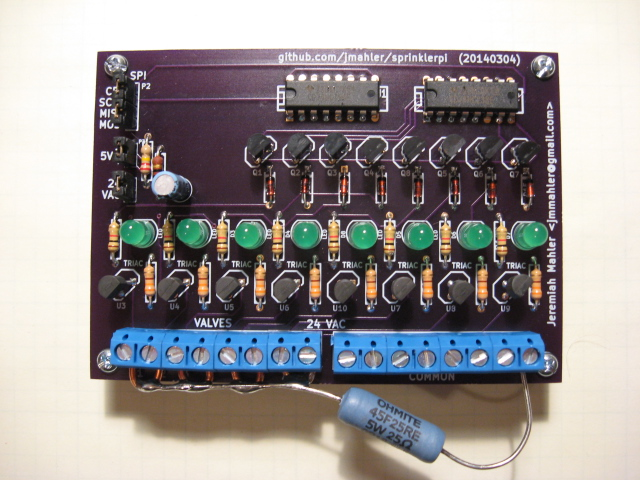
\includegraphics[scale=0.6]{img/control_driver_tb_02.jpg}
\end{center}
\caption{Control driver with test bridge (bottom) installed.}
\label{fig:cdbridge}
\end{figure}

\begin{framed}
\textbf{IMPORTANT}: The DC voltage has been changed
from 5V to 3.3V.
The label on version 20140304 of the control driver PCB still
refers to 5V despite this change.
\end{framed}

\begin{enumerate}
\item Equipment Required
	\begin{itemize}
	\item SprinklerPI power supply module (revision 20140304).
	\item 110 volts AC power supply (standard U.S.).
	\item 110 volts AC to 24 volts AC power adapter.
	\item Digital multi meter.
	\item RasberryPI.
	\item Jumper wires.
	\item Control/Driver test bridge (25 $\Omega$, 5 Watt)
			(Figure \ref{fig:cdbridge}).
	\end{itemize}
\item Input
	\begin{itemize}
	\item User turns valves on using command line interface.
	\end{itemize}
\pagebreak
\item Output
	\begin{itemize}
	\item Green LED on for valve which is on.
	\item $9.5\pm0.5$ volts AC across test bridge resistor when on.
	\end{itemize}
\item Test Description \\

These tests verify that each of the eight circuits can be turned
on and that they can adequately drive a load.
The operation of each circuit can be seen by the green LED indicator
which is on when that valve is on.
The load is checked by measuring the voltage drop across the
resistor of the test bridge (Figure \ref{fig:cdbtest}).
The voltage drop should be $9.5\pm0.5$ volts AC which corresponds
to a current draw of $380$ mA for the $25 \Omega$ load.

\begin{figure}[htbp!]
\begin{center}
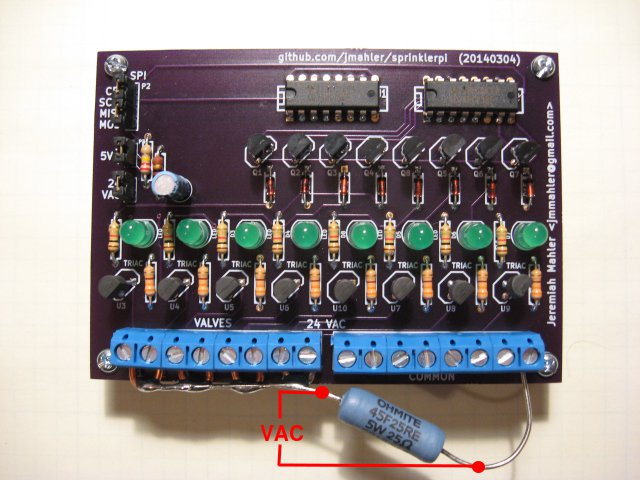
\includegraphics[scale=0.6]{img/control_driver_tb_03.jpg}
\end{center}
\caption{Voltage test point for control driver test bridge.}\label{fig:cdbtest}
\end{figure}

Once logged in to the RasberryPI each valve can be turned on by
running the \verb+water+ command.

\begin{verbatim}
rasberrypi:~$ water "1"
rasberrypi:~$ water "2"
rasberrypi:~$ water "3"
rasberrypi:~$ water "0"  # turn off
\end{verbatim}

See \verb+water -h+ for more info.

\pagebreak
\item Test Results \\
	\vspace{0.2in}
	\begin{tabular}{|l|l|l|l|l|}
		\hline
		& LED on? & Voltage Drop    & Pass/Fail & Results/Data\hspace{2in} \\
		&         & $9.5\pm0.5$ VAC & & \\
		\hline
		1 &&&& \\
		\hline
		2 &&&& \\
		\hline
		3 &&&& \\
		\hline
		4 &&&& \\
		\hline
		5 &&&& \\
		\hline
		6 &&&& \\
		\hline
		7 &&&& \\
		\hline
		8 &&&& \\
		\hline
	\end{tabular}
\end{enumerate}
% }}}

%\section{Other Testing}

% {{{ User Interface
\clearpage
\subsection{User Interface}

\begin{enumerate}
\item Equipment Required
	\begin{itemize}
	\item Computer with web browser and network connection.
	\end{itemize}
\item Input
	\begin{itemize}
	\item Turn valve on/off.
	\item Check status of valve.
	\item Schedule time and duration to run valve.
	\end{itemize}
\item Output
	\begin{itemize}
	\item Valves go on when commanded.
	\item Status of operating valve shown when on.
	\item Scheduling a time and duration works as expected.
	\item Pass: Valves operate according to the commands.
	\item Fail: Response is not expected.
	\end{itemize}
\item Test Description \\

The basic commands given through the web interface are:
on/off valve, show current status, schedule a time/duration.
These tests verify these operations.

\item Test Results \\
	\vspace{0.25in}
	\begin{tabular}{|l|l|l|l|l|l|c|}
		\hline
		\multicolumn{7}{|c|}{Valves On/Off} \\
		\hline
		\# & On? & On Status? & Off? & Off Status? & Pass/Fail & \hspace{0.7in}Notes\hspace{0.7in} \\
		\hline
		1 &&&&&& \\
		\hline
		2 &&&&&& \\
		\hline
		3 &&&&&& \\
		\hline
		4 &&&&&& \\
		\hline
		5 &&&&&& \\
		\hline
		6 &&&&&& \\
		\hline
		7 &&&&&& \\
		\hline
		8 &&&&&& \\
		\hline
	\end{tabular}

	\vspace{0.25in}
	\begin{tabular}{|l|l|l|l|l|}
		\hline
		\multicolumn{5}{|c|}{Schedule} \\
		\hline
		\# & Time Start & Time End & Pass/Fail & \hspace{0.5in}Notes\hspace{0.5in} \\
		\hline
		& now & now + 1 minute & & \\
		\hline
		& now & now + 5 minute & & \\
		\hline
	\end{tabular}

\end{enumerate}

% }}}

\end{document}

